\documentclass[journal,final,letterpaper,11pt]{IEEEtran}
\usepackage{multirow}
\usepackage{url}
\usepackage{cite}
\usepackage{graphicx}
\usepackage{algorithmic}
\usepackage{enumerate}
\begin{document}
\title{How to Cheat in Puzzles and Dragons}
\author{Amanda~Chow, Ted~Li, and~David~Zeng}
\markboth{CS 221 Final Paper, Autumn 2015}{}
\maketitle

\section{Introduction}
\IEEEPARstart{P}{uzzles} and Dragons (PAD) is one of the most popular games on both  Android and iOS. It takes a unique approach to mobile gaming, combining aspects of both RPGs and puzzle games to create a game where you pick a team of monsters and level them up by battling evil monsters. During the battles, you play a matching puzzle game, which will be focus of our project.

\begin{figure}[h]
\centering
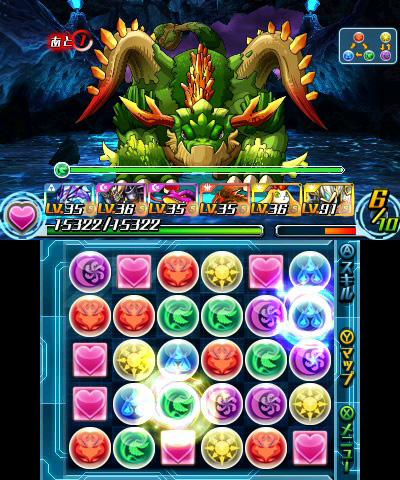
\includegraphics[scale=0.5]{pad.jpg}
\center{\textbf{Fig. 1} Example PAD Board}
\end{figure}

The puzzles in the game present you with a randomized puzzle board (shown above) with $5$ rows and $6$ columns. In most battles, each of these spaces contains one of six orbs: Fire, Water, Grass, Light, Dark, and Heart. To begin solving the puzzle, you select an orb and drag it. As you drag it through other orbs, the other orbs will swap locations with the orb you are dragging, effectively pushing the orbs in your path behind you. The goal of dragging the orb around is to position other orbs so that you form groups of orbs of the same color. Once you let go of your selected orb, or reach a $4$ second limit, your turn is completed. The game then finds adjacent groups of orbs of the same color and gives you a score based on the size of these groups and the number of groups.

\section{Gameplay Implementation}
Our project focuses on creating a AI designed for cheating on the puzzles. We decided to frame the PAD puzzle as the following problem: given a limited number of moves, what is the highest scoring path one can achieve on a random board? The \textbf{inputs} of our AI would be a $5 \times 6$ grid of orbs, represented as integers $0$ through $5$, and the \textbf{outputs} would be an optimal path, represented as a list of $(x,y)$ coordinates.

\subsection{Restrictions on the Game}
PAD allows the player unlimited time to think about the board, but only four seconds to drag around an orb. For a good player, this usually equates to dragging the orb around $40$ spaces after some initial thought to plan the path. Therefore, the speed that our AI works at it not a priority. However, for our AI to fairly emulate what is possible for a human, it will also need to limit the number of moves it can execute on a turn to $40$. In addition, PAD also allows the player to drag an orb in all $8$ ordinal directions, but for most human players, diagonal dragging is very difficult to execute accurately, especially given the time limit and the small size of the mobile screen. Therefore, we chose to also limit our AI to only make moves in $4$ ordinal directions: up, down, left, right.

\subsection{States and Actions}
We defined our states as any representation of the current board, where each of the 30 entries has a value of 0 to 5. In each of our states, we not only have the board matrix representation, but we also have the coordinates to our current orb. Actions are defined as any direction, \texttt{U}, \texttt{D}, \texttt{L}, and \texttt{R}, which correspond to moving our current orb $(0, 1), (0, -1), (-1, 0), $ and $(1, 0)$. When we perform an action, we update our state by swapping the value of our current location with the value of our next location, which is our current orb's location plus the move. We then define the location of our current orb as the new location.

\subsection{Scoring Method}
To properly evaluate the performance of our AI, we need a metric to evaluate the PAD puzzle board. Our full evaluation metric, which we will call \texttt{PADScore} performs the following algorithm based on the Puzzles and Dragons scoring mechanic \cite{1}.
\begin{enumerate}
\item Find all continuous groups of 3 or more orbs in single rows and columns.
\item Combine groups of the same color that either intersect or are adjacent.
\item Each group is given a score of $1 + \frac{1}{4}(\mbox{size} - 3)$. \item Sum the scores for each group.
\item Multiply by the sum by the combo multiplier, given by $1 + \frac{1}{4}(\mbox{\# of groups} - 1)$.
\end{enumerate}
The actual PAD game also takes into account orb types and how they interact with the offensive attributes of your team and the defenses of the actual monsters, but the pure mathematical score of the board is computed in an identical manner. 

To speed up the scoring computation, we also define a score heuristic, which we call \texttt{GroupCount}. This  is given by
\begin{enumerate}
\item Count the number of continuous groups of 3 or more orbs in single rows and columns.
\end{enumerate}
This captures a good estimate of the full score, without having to run the intersection logic between all the groups. However, this scoring method does not fully emphasize the impact of getting larger combos. For example, going from three groups of 3 to four groups of three will increase \texttt{GroupCount} from 3 to 4. However, the actual \texttt{PADScore} will increase from 5.25 to 8.

In order to assign a more accurate fitness score, we will define another score heuristic, which we call \texttt{ScoreIndividuals}. This is given by
\begin{enumerate}
\item Count the number of continuous groups of 3 or more orbs in single rows and columns.
\item Each group is given a score of $1 + \frac{1}{4}(\mbox{size} - 3)$. 
\item Sum the scores for each group.
\item Multiply by the sum by the combo multiplier, given by $1 + \frac{1}{4}(\mbox{\# of groups} - 1)$.
\end{enumerate}
While it typically ends up overestimating the score since intersecting groups are not combined, it still emphasizes the importance of having a large combo, especially when we start getting to higher scores.

\section{Prior Work on PAD Solvers}
There are various cheating applications for the Android and iOS versions of PAD that take a screenshot and overlay a high scoring path on top of the image. However, none of these applications publish their source code or document their approaches. 
We did find a similar PAD web application, pndopt (Puzzles and Dragons Optimizer) \cite{2}, that runs a beam search algorithm. Pndopt banks off the idea that paths are built off of incremental components that line up orbs. At each step, pndopt retains the $K$ best paths of length $n$, and then augments these paths by one additional action. The scores for these augmented paths are then recomputed, and the best $K$ are retained for the next iteration. The algorithm will explore paths up to some fixed length $N$. Though quite a simple algorithm, pndopt proves to work fairly well. As such, we decided to us pndopt as our ``oracle''.

Evaluating the outputs with our scoring metric, over 100 randomized trials, pndopt averaged a \texttt{PADScore} of $15.52$ with an average path length of $28.57$, which roughly corresponds to aligning $6$ groups of three orbs. 

The benefit of a simple beam search algorithm is that it runs quite fast and will usually preform well. Of course, there are certain board configurations on which a greedy algorithm may perform extremely poorly, but to function as a cheating application, speed is of the essence so that users do not get impatient with the app. For our project, we decided to look at a variety of unsupervised algorithms for finding PAD solutions, which are detailed below.

\begin{enumerate}
\item a randomized baseline
\item hill-climbing, an aggressive search algorithm that only accepts local improvements, described in section 4.4 of \cite{3}. We worked with two variations of this algorithm, steepest ascent hill-climbing and simulated annealing
\item genetic algorithms, a randomized search algorithm that emulates the behavior of natural selection, described in detail in chapter 1 of \cite{4}
\end{enumerate}

The remainder of this writeup describes our various approaches in full detail, the implementation choices we made, and the results and conclusions we drew from each. 

\section{Baseline Implementation}
Our baseline AI implementation is based on a player making random moves. It performs the following algorithm.
\begin{algorithmic}[1]
\FOR{$i=1$ to $1000$}
  \STATE reset the board to original state
  \STATE pick a random orb to start
  \STATE $S_i :=$ score of board
  \STATE $P_i :=$ empty path
  \FOR{$j=1$ to $40$}
    \STATE drag the orb in a random direction
    \STATE $S :=$ score of board
    \IF{$S > S_i$}
      \STATE $S_i := S$
      \STATE $P_i :=$ path so far
    \ENDIF
  \ENDFOR
\ENDFOR
\RETURN $\max_{i}\{S_i\}$ and corresponding path $P_i$
\end{algorithmic}
We generated $100$ boards at random and ran our baseline algorithm on the boards and recorded its performance. The baseline achieved a \texttt{PADScore} of $7.38$ using an average path length of $25.31$. This roughly corresponds to the baseline algorithm being able to align $4$ groups of three orbs each.

\section{Approach I - Greedy Hill Climbing}
After the baseline, we started with a greedy player implemented using hill climbing. The idea was to only take moves that increase or maintain the current score. We explored several different variations of hill climbing, with varying levels of greediness, and the major variations are reported below.

\subsection{Steepest Ascent Hill Climbing}
To set a baseline for hill climbing, our first hill climbing player was the greediest - not only did it only choose moves that increase or maintain score, it actually chose the move that increased the score the most. In the case where multiple moves can result in the same maximum possible immediate score, the player chooses one of those moves at random. If all possible moves decrease the score, then the player has reached a local maximum score, and stops. The player would take these moves as described to increase the immediate score as much as possible, thus tending toward local maxima. The algorithm is performed as follows:

\begin{algorithmic}[1]
\STATE \textbf{input}: board $B$
\STATE pick a random orb to start
\STATE $P :=$ empty path
\FOR{$j=1$ to $40$}
  \STATE $M :=$ moves with best immediate score
  \IF{$M$ is empty}
    \STATE break
  \ENDIF
  \STATE $A :=$ random move from $M$
  \STATE Take move $A$
  \STATE $P :=$ path so far
\ENDFOR
\RETURN board score of $b$ and path $P$
\end{algorithmic}

This player averaged a \texttt{PADScore} of $3.32$ with an average path length of 40.7 over 1000 random starting boards. This is roughly equivalent to aligning 2 groups of three orbs each. 

As expected, this player is too immediately greedy and does not perform very well. Examining several games in detail, we noticed that the player often gets stuck at local maxima, stepping back and forth endlessly between states that have equal scores until it runs out of moves - hence the path length of 40.7. Aside from the states explored during the hill climb, the player unfortunately never has the chance to explore more of the state space - which is generally advantageous for most AI's and increases the likelihood of finding higher local maxima.

\subsection{Simulated Annealing}
In order to balance the trade-off between greediness and exploration of state space, we then decided to incorporate simulated annealing into our hill climbing player. Rather than always choosing moves that increase or maintain the score as much as possible, at each state, there is a probability $p$ that the player will chose any random move that \textit{decreases} the score. (If there are no moves that decrease the score, then the player randomly chooses any move). The rationale behind this choice is that it gives the player a chance to explore the state space more, and increases the likelihood of stumbling on a state that leads to better scores. In other words, it occasionally strays off the hill climb and makes sacrifices the score in hopes of discovering new, taller "hills" to climb. 

To give the player a chance to explore the state space, we let it play 1000 times from the same starting board. Each play, it generates a random starting position and makes moves from there. Over the 1000 different plays, we take the best score and return its corresponding path. Given a randomly generated starting board $B$ and a probability $p$ of taking worse moves, the algorithm works as follows:

\begin{algorithmic}[1]
\STATE \textbf{input}: board $B$, probability $p$
\STATE $S := 0$
\FOR{$i=1$ to $1000$}
  \STATE Start at original board $B$
  \STATE pick a random orb to start
  \STATE $P_i :=$ empty path
  \FOR{$j=1$ to $40$}
    \STATE Pick random real $x$ in [0, 1]
    \IF{$x < p$}
      \STATE $M :=$ moves that decrease score
      \STATE $A :=$ random move from M
    \ENDIF
    \IF{$x > p$ or $M$ was empty}
      \STATE $M :=$ moves with best immediate score
      \STATE $A :=$ random move from M
    \ENDIF
    \STATE Take move $A$
    \STATE $P_i :=$ path so far
  \ENDFOR
  \STATE $S_i :=$ score of board
  \IF{$S_i > S$}
    \STATE $S := S_i$
    \STATE $P := P_i$
  \ENDIF
\ENDFOR
\RETURN score $S$ and path $P$.
\end{algorithmic}

The choice for the value of $p$ depends on how much exploration of the state space we want. The first greedy hill climber essentially operated with $p=0$, always opting for the best immediate score, but hardly exploring the state space. We started with a probability of 0.2, and had the player find solutions to 100 randomly generated starting boards. Over these 100 boards, the player averaged a \texttt{PADScore} of 7.9, and an average path length of 38.57. This corresponds to roughly 4 groups of three orbs each.

This player was less greedy and performed significantly better than the greediest hill climber. However, it was still a long ways from the oracle, so we set out to find the best value for $p$. After trial and error, we found the best value for $p$ to be approximately $p=0.08$. A player with $p=0.08$ could produce an average score of 8.5 with an average path length of 40.8 over 100 boards. This corresponds to roughly 2 groups of three orbs each and 2 groups of 4 orbs each.

This was the best value we were able to achieve using hill climbing with simulated annealing. This player performs barely better than our general baseline (the random player) due to its nearsightedness, in that it only aims to maximize the immediate score after one move. Even with simulated annealing, the amount of exploration of the state space is very limited - the state space is simply too large to explore fully. Given the limitations of hill climbing in such a large state space, our next step was to employ search techniques with local optimizations.

\section{Approach II - Genetic Algorithms}
Genetic algorithms are based on the principle of natural selection. We encode members of our search space as if they were DNA strings, and emulate selection, reproduction, and mutation of a population over time, in hopes that the population grows stronger and leads us towards better solutions. The motivation to try genetic algorithms for PAD comes from two sources: 
\begin{enumerate}
\item The goal of solving PAD is to find an optimal path of some maximum length. Searching over this state space easily translates to searching over string representations of paths, which is in line with the language of genetics.
\item The human approach to PAD involves recognizing small patterns or orbs to line up orbs one group at a time \cite{5}. The small sequences represent ``genes'' of the path, and the solution essentially comprises of stringing together the right genes. 
\end{enumerate}

\subsection{Genomic Path Representation}
The first step in making a genetic algorithm is to design a genomic string representation of the search space. A path in PAD essentially comprises of first picking a starting orb, and then making up, down, left and right movements. For a given starting orb, all paths from that orb can simply be encoded as strings of four characters, each representing a directional action: \texttt{U}, \texttt{D}, \texttt{L}, and \texttt{R}. Genetic algorithms work best when all genomes of the population have the same length. In order to allow variation in path length while still keeping the genomic length constant, we also introduced a pause action \texttt{P}. 

\subsection{PAD Genetic Algorithm}
A genetic algorithm for PAD works as follows:
\begin{algorithmic}[1]
\STATE \textbf{input}: board $B$, starting location $(r, c)$
\STATE \textbf{parameters}: population size $S$, genome length $L$, number of generations $G$
\STATE $P$ := list of $S$ random genomes of length $L$
\FOR{$i=1$ to $G$}
  \STATE assign fitness score to each member of $P$
  \STATE $C$ := empty list for offspring
  \FOR{$j=1$ to $S$}
    \STATE \textbf{selection}: pick members of $P$ with probability proportional to fitness score
    \STATE \textbf{reproduction}: generate $1$ offspring based on the members selected
    \STATE \textbf{mutation}: randomly modify the offspring
    \STATE add the offspring to $C$
  \ENDFOR
  \STATE $P$ := $C$
\ENDFOR
\RETURN path with highest score in $P$
\end{algorithmic}

There are many schemes to try for selection, reproduction, and mutation. We explored different combinations of these
\subsubsection{Selection} 
The fitness of each path is defined as how well the path groups together gems, quantitatively defined as the score of the board obtained by following the path (scored using \texttt{GroupCount}). Paths that produce more groups are favored in selection. In particular, paths that run off the board will receive a score of $0$ and will not be viable for selection.
\subsubsection{Reproduction}
The basic implementation picks $2$ parents during selection (with probability of selection of each parent based on its fitness), reproduces using single point crossover. Single point crossover is defined as the following:
\begin{enumerate}[{i.}]
\item Given two parents, pick a split point at random
\item Take the genetic info of one parent before the split, and one parent after the split
\begin{verbatim}
parent 1:  UDLRU|DLRUDLRUDLR
parent 2:  LRDUL|RDULRDULRDU
----------------------------
offspring: UDLRU|RDULRDULRDU
\end{verbatim}
\end{enumerate}
\vspace*{0.1 in}
\subsubsection{Mutations}
To increase the diversity of our population (and thus explore the state space more), we can introduce random mutations into children by toggling a move with a small probability.

\subsection{Initial Results and Iterations}
This implementation of the genetic algorithm achieves an average \texttt{PADScore} of $9.94$ with an average path length of $28.80$ over $100$ random boards using a randomized starting location for each board. For this run, we use a population size of $10000$ genomes, each of length $30$ (instead of $40$), and iterate the genetic algorithm for $50$ generations.
This corresponds to our algorithm producing $5$ groups of three orbs each, and improvement of one group over the baseline method. 

\subsubsection{Starting in Center} We noticed that runs of our algorithm that started in the center of the board as opposed to edges produced higher scores in the end. If we only start our genetic algorithm on orbs that are not in the outer ring, we achieved a \texttt{PADScore} of $10.73$ over our random boards, with all other parameters held constant. This is likely to do with the fact that paths that start on the edge are more likely to run off the board and produce illegal paths, which have a fitness of $0$ under our scheme.

\subsubsection{Double Point Crossovers} We also tried other variations of the reproduction scheme. Rather than single point crossovers, we tried double point crossovers, which are defined as the following: 

\begin{enumerate}[(i.)]
\item Given two parents, pick two split points at random
\item Extract the section of one parent between the split points, and replace the corresponding section of the other parent with this foreign DNA.
\begin{verbatim}
parent 1:  UDLRU|DLRUDL|RUDLR
parent 2:  LRDUL|RDULRD|ULRDU
----------------------------
offspring: UDLRU|RDULRD|RUDLR
\end{verbatim}
\end{enumerate}
\vspace*{0.1 in}
Using double point crossovers for reproduction did not improve the performance. Over 100 random starting boards, it achieved an average \texttt{PADScore} of $10.54$. This is likely because double crossovers do not introduce that much variation into the population (like single crossovers), and examining the population after 50 generations confirms this fact. Regardless of whether we used single or double point crossovers, the population becomes very homogeneous after 50 generations. In fact, on some runs the entire population had converged to one genome.

\subsubsection{Mutations} In an attempt to increase the diversity of our population, we introduced random mutations into the population. Whenever two parents reproduce to make a child, each move in the genome was toggled with a $1/$\verb+(genome length)+ and with a $5\%$ chance. Introducing both of these mutation rates also did not improve our player. This is likely because of how a single move in Puzzles and Dragons will affect all of the following moves as well - for example, flipping a direction will displace all future moves by two spaces. This means that almost all of our mutations ended up pushing our paths off of the board and then getting assigned a score of 0. And in the rare cases where the paths still exist, they typically will decrease the score, since the rest of the path, which has been selected for through our AI, is also displaced, and thus, are no longer necessarily good.

\subsubsection{Starting Position} Because we represented a path as a series of moves, the performance of the path is relative to the starting position. The optimal path itself also depends the start position, so we tried running the algorithm once for each starting position on the board and taking the best of those runs. As expected, this player performed slightly better than before, achieving an average score of 11.41 over 100 boards. This improvement demonstrates that the way the player refines the path is really dependent on the start position, as the best path starting at one position likely results in very low scores (or falls off the board) starting from any other position on the board. Having this extra information improved our player's performance and required only a polynomial time increase in runtime.

\subsection{Analysis and Limitations}
Overall, this genetic algorithm works much better than hill climbing, because it is much better at achieving local optimizations. In particular, there are certain sequences of moves that work well in PAD, depending on the starting configuration, such as rotating a group of four gems arranged in a square (eg. \verb+URLD+). These sequences of moves are the genes that our algorithm locally optimizes. Looking at the best sequences produced by our player showed that our algorithm was successful at identifying these genes - there were many such sequences in the best paths.

However, this genetic algorithm has several limitations that prevented further improvement when we attempted variations such as double point crossover. First, the way the path is modeled as a gene (a random sequence of \verb+U, D, L+, and \verb+R+ means that the much of our population consists of paths that go off the board and yield a score of 0, even if we start in the center squares as above. This means the genes contained by these paths are lost, and such a frequent die-off of paths heavily decreases the diversity of our population from generation to generation. An analysis of the populations showed that around $90\%$ of paths in the first generation fall off the board. Of course, this percentage decreases from generation to generation, as the population evolves to become more fit, but this initialization of a population that is effectively $90\%$ dead severely limits the diversity that our population has to work with right from the start.

Even at a more fundamental level, the way the path is modeled as a gene lacks information about the positions of each move. This information is crucial to the player because each position on the board has a color, and the sequence of moves that aligns gems at one specific location of the board, if performed at a different location on the board, will align different gems and likely not perform as well. As proof, our player that runs the algorithm once for each starting position performs better because it has information about the positions of the path. 

Given these limitations, we were faced with the task of restructuring our genetic model with two goals:
\begin{enumerate}[(i)]
\item Giving our player information about the positions - describe paths in more detail by specifying board position(s).
\item Maintaining the diversity of our population - for instance, by reducing the die-off rate.
\end{enumerate}

\noindent Before, the limited descriptiveness of paths and the limited diversity of our population limited the performance of our player. Together, these changes should give our player a much higher potential to score better.

\section{Approach III - Genetic Algorithms with Positions}
As an improvement on our previous player, this player is designed to strategically use the board positions to inform decisions. The idea is to localize sequences of moves to specific board locations, because an optimal path really consists of these local optimizations that rearrange orbs with other closely orbs.

\subsection{Path Representation}
The first major change is the way that paths are represented - each particular move of the path has a starting location and a direction \verb+U, D, L+, or \verb+R+. Thus, a path can be represented as a list of ordered pairs of (start location, direction). Although only the start position of the entire path and direction of each move are needed to represent our graph, it was more practical for us to store the start location and direction of every move (so that we don't have to recompute the entire path every time two parents reproduce using our new crossover method, explained below).

Because of this new representation, we only initialize paths that stay on the board, so $0\%$ rather than $90\%$ of our original population is effectively dead. To keep this die-off rate from generation to generation at $0\%$, we also have a new crossover method that simultaneously uses our new information about board positions to only produce child paths that stay on the board. 

\subsection{New Crossover Method without Frequent Die-off}
The crux of this new player lies in the way that parent paths reproduce using the new information about positions. Here, we introduce a variant of the one-point crossover that uses the physical positions of the paths to produce offspring: 

\begin{enumerate}[{i.}]
\item Given two parent paths, pick a split position that both parents intersect at (denoted by the green square in f). If the parents intersect at multiple points, pick one intersection point at random. If the parents don't intersect, they don't produce offspring.
\item Swap the end portions of the paths after the split point with each other. Pick one as a child. This crossover is illustrated below:
\end{enumerate}

\begin{figure}[h]
    \centering
    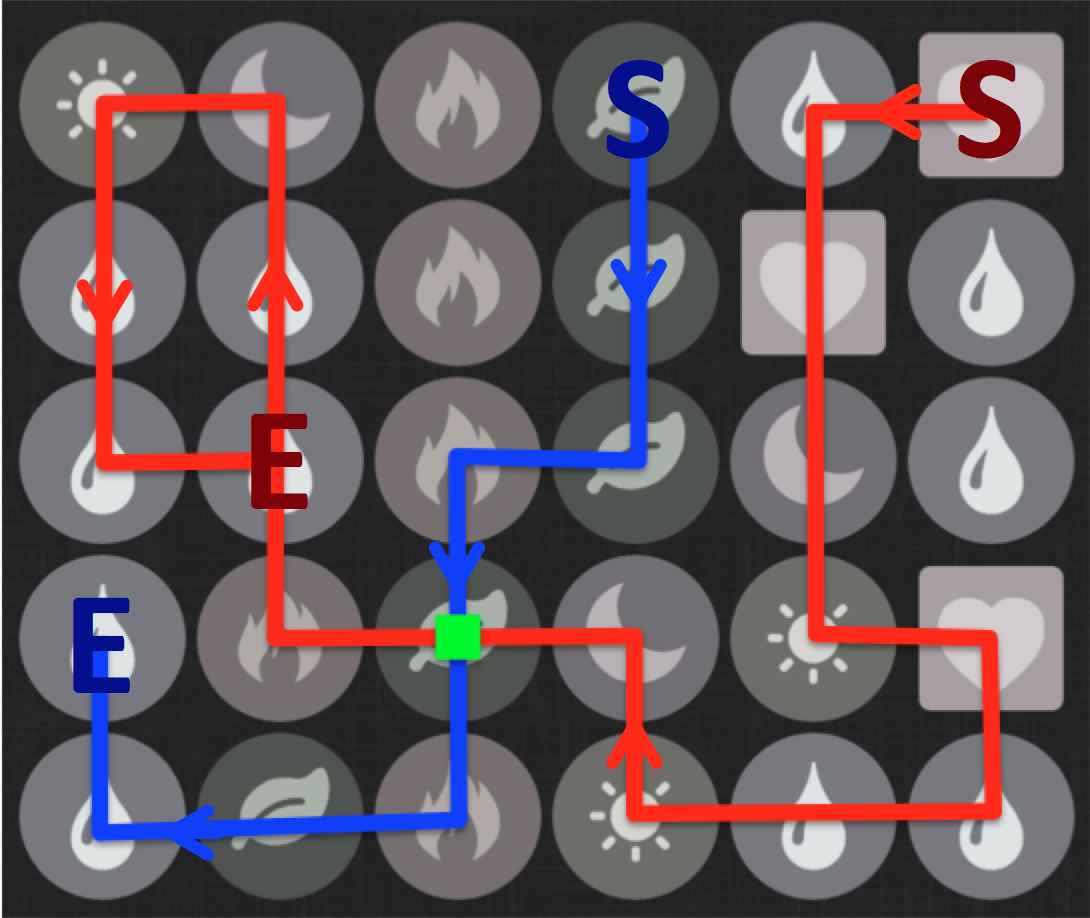
\includegraphics[width=0.3\textwidth]{before.png}
    \center{\footnotesize{\textbf{Fig. 2a}: Before crossover. Split point denoted by green square.}}
    \label{fig:before}
\end{figure}

\begin{figure}[h]
    \centering
    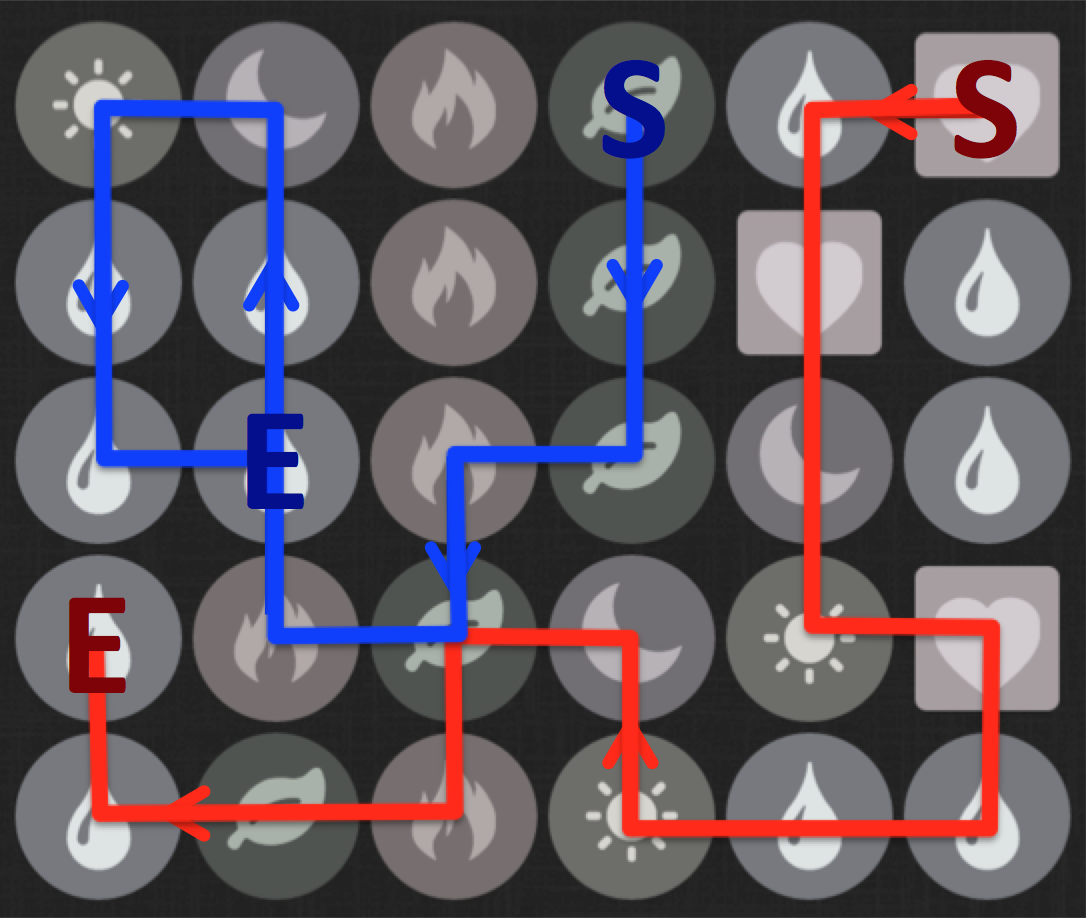
\includegraphics[width=0.3\textwidth]{after.png}
    \center{\footnotesize{\textbf{Fig. 2b}: After crossover. Paths have swapped before/after split point}}
    \label{fig:after}
\end{figure}

This crossover method has a number of advantages for this genetic algorithm. First, because it only uses existing portions of paths, the children paths produced always stay on the board, as long as the starting population only has paths that stay on the board. Given that we initialize our population with legal paths (paths that stay on the board), this crossover method will eliminate the frequent population die-off that our previous player experienced, resulting in a more diverse population and therefore more potential to find better paths.

In addition, because this crossover method picks a common position rather than a common move index, it has a more suitable idea of a gene as a localized series of moves rather than a position-independent series of moves.

\subsection{New Genetic Algorithm}
With this new representation of the game, some minor modifications were necessary. First of all, as explained before, this new path representation takes into account the position at every move - therefore, there is no longer a need to run the algorithm once for different starting positions. When initializing our population, starting positions are chosen at random, and legal moves are chosen from there. The population is evenly distributed among starting positions, and the evolutionary algorithm will select for the fittest starting positions and paths from there. Thus, only one starting population is required for a board, rather than one starting population for each start position on the board.

In addition, this implementation produces variable length paths, and inevitably some path lengths exceed our maximum of 40 moves. To control the length of paths, we redefine the parameter $L$ as the length of the paths that we initialize in our starting population. Setting this $L=30$ produces optimal paths that vary in length from 15-50 moves, which are very reasonable path lengths.

This new genetic algorithm works as follows:

\begin{algorithmic}[1]
\STATE \textbf{input}: board $B$
\STATE \textbf{parameters}: population size $S$, starting genome length $L$, number of generations $G$
\STATE $P$ := list of $S$ random genomes of length $L$
\FOR{$i=1$ to $G$}
  \STATE assign fitness score to each member of $P$
  \STATE $C$ := empty list for offspring
  \FOR{$j=1$ to $S$}
    \STATE \textbf{selection}: pick members of $P$ with probability proportional to fitness score
    \STATE \textbf{reproduction}: generate offspring by crossing locations
    \STATE \textbf{mutation}: randomly modify the offspring
    \STATE add the offspring to $C$
  \ENDFOR
  \STATE $P$ := $C$
\ENDFOR
\RETURN path with highest score in $P$
\end{algorithmic}

\subsection{Initial Results and Iterations}
We ran this player with the same hyperparameters as before: a population size of 10000 genomes evolving through 50 generations, as well as the new parameter of initial genome length of 30 moves. This new player delivered much better results. Over 100 boards, it achieved an average score of 13.60, with average path length 25.3. As expected, it was better at identifying genes as localized sequences of moves and aligning nearby groups of orbs.

\subsubsection{Increasing Population Size}
First, we tried increasing the population size from 10000 to $100,000$. This slowed down the algorithm but improved the average high score to 15.86 with an average path length of 21.1.

\subsubsection{Independent Runs}
We also tried running 10 independent runs of the algorithm for each board, where each run has a different randomly initialized starting population. The optimal path was taken as the best path produced from among the runs. With this modification, our player improved by several points and produced an average high score of 15.69 with average path length of 25.9.

\subsection{Analysis}
Overall, this algorithm is much better at isolating genes and making local orb swaps than the previous player. Increasing the initial population size and running several different runs had an equivalent effect of increasing population variation, thereby increasing the score from about 13.6 to about 15.8. 

However, we are still a few points behind our oracle for specific boards. This is likely because our algorithm doesn't take into account the swaps - as moves are made, the board changes, and a gene that worked well on the starting board may not work well after a few genes have already operated on the starting board. Examining example boards with the oracle reveals this as well. Consider the board below:

\begin{figure}[h]
\centering
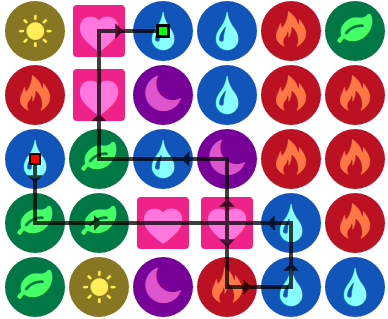
\includegraphics[scale=0.5]{Pad_Analysis_Path.png}
\center{\textbf{Fig. 3} Example board with oracle's solution}
\end{figure}

The oracle's path for this board yields a score of 18.75, while our path yields a score of 16.3125 (it starts at (2,0) and follows the moves \verb+RULDDRURRDDRULURUULD+). The oracle's path only traverses each position at most twice, taking advantage of knowledge about the start state. However, our path traverses some locations more than twice. The more times a particular location is traversed, the more the board deviates from the starting board, and the less optimal our genes are. One limitation of our model is that it doesn't take these board modifications into account as they happen. In theory, storing the board configuration at each move would give our model more information and improve the performance; however, in practice, the state space would become exponentially larger and too expensive to explore in a reasonable amount of time.

\subsection{Ideas for Improvement}
Over the past few weeks, we have made many improvements to our AI. However, here are some more ideas that we think may improve the performance
\begin{enumerate}
\item Add even more variability. The previous genetic algorithm player did not benefit from mutations. However, this model has the potential to, if we are able to define exactly how to mutate a path. We are still faced with an issue of a nearly completely homogeneous population after many generations. One possible way we might want to diversify our population may be to randomly generate new paths and include them to our population in every generation.
\item Select better initial population. Because our initial population is completely random, we often face issues with taking too long to find a good answer and suffer in solving very easy boards (more detail about this in error analysis). However, if we are able to add a few paths to our population that are greedy-searches or something similar, we may be able to get a good starting point to build our population on.
\end{enumerate}

\section{Error Analysis}
Overall, there were many error points that we identified through our different implementations. As mentioned earlier, both of our greedy algorithms were far too greedy and did not look far enough ahead. As a result, these both suffered from local maxima and did not end up exploring very much of the board. 

When we moved onto genetic algorithms, we faced a new set of errors. One of the first steps in our algorithm was to generate a population of paths. Not only were our paths long, but we were also playing on a relatively small board. After testing, we found that around $90\%$ of our paths ran off the board and returned scores of 0. This in turn pruned off most of our population at the start. As a result, we lost a lot of our genetic diversity, negatively impacting our scores. 

In our second attempt at a genetic algorithm, we changed our paths so that they would never fall off the board. In addition, we managed to avoid falling into local maxima by looking at the final score only, in terms of evaluating our paths. However, we still have many lingering error points that we've identified in our final implementation.

\subsection{Performance on "Good boards"}
Over many randomized maps, our AI performs at a level comparable to our oracle. However, while testing, we noticed that occasionally our AI would output significantly lower scores. Looking more closely at the maps, these discrepancies are most common when the maps are relatively "easy" to score well on. It's not that our AI performs worse than usual on these maps - it's that it doesn't perform well enough. Take the board shown below for example. On this board, with 30 iterations, one for each starting position, our AI achieved a maximum \texttt{PADScore} of 12.6875 and an average of 11.65. On the other hand, the oracle returned a \texttt{PADScore} of 27. While our AI was only able to find five matches, the oracle was able to find eight. 

\begin{figure}[h]
\centering
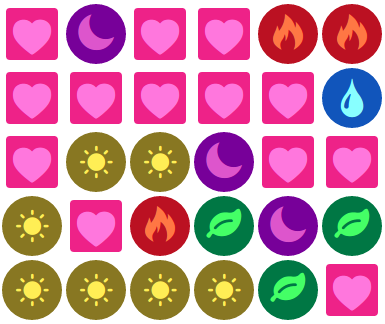
\includegraphics[scale=0.5]{Pad_Board_1.png}
\center{\textbf{Fig. 4} Example of a Good Board}
\end{figure}

The cause of this error seems to come down to our implementation. When given a relatively easy map, the oracle, which uses a greedy algorithm, has a clear direction. Since the map is so simple, the greedy algorithm is not punished for not looking ahead far enough. On the other hand, our genetic algorithm generates paths on a holistic scale, evaluating only based on the final score. We hoped that even with this approach, good sections of our paths would eventually mutate with each other and form a final, successful path. However, since our initial paths are random and we are limited by population size and generations, we ultimately end up with average paths that give us scores near our overall mean. Simply put, our algorithm seems to be great at consistently getting decent scores, but fails to score very well on easy maps.

\subsection{Local Maxima}
Another major flaw of our algorithm is that after many generations, we end up with an almost homogeneous population. This lack of diversity then can lead to us getting stuck at local maxima, because regardless of what kind of how many crossovers we do, the children will always be the same. We have tried fixing this with random mutations, but they are too scarce and often do not have a significant enough of an impact in order to change up our population. In addition, with the structure of our second genetic algorithm, a simple mutation in the middle of a sequence can throw off an entire path and lead to issues with staying on the board.

\subsection{Runtime}
A common issue that many genetic algorithms including our own face is runtime. Because we start at each of the 30 locations, have a large population size of 10,000, and go through 50 generations, we end up spending a lot of time doing calculations. We have tried to scale down our numbers in order to speed up our AI, but have found that large changes severely negatively impact our performance.

\subsection{A Constantly Evolving Board}
The current genetic algorithm model is made to identify specific "genes," which represent short sequences of moves that are good for our board and then hopefully pass these genes on to their children. However, this faces a problem when we use this idea over many moves. This because in Puzzles and Dragons, the board is constantly evolving. If we are in the top left corner at the start, and at some point in our turn we find ourselves in the top left again, it's very likely that the board has transformed. Consequently, that means that what constituted a good sequence of moves the first time we were in that location, might not be a good sequence of moves now. What this means, is that not only is the location of genes important, but the time and the neighboring blocks when we look at genes, is important. However, our model does not account for this and therefore will often pass on good genes into a different context and have it perform poorly.

\section{Conclusions}
Overall, we found that of all of our AI, the Genetic Algorithm with Positions was the most successful. Our greedy search algorithms both face the issue of hitting local maxima too soon - even with simulated annealing, these were unable to look far enough ahead into the future to make beneficial moves and increase their score above even the baseline. The fist genetic algorithm fixed many of these problems, though it was still faced with a few issues, namely genetic diversity due to paths having scores of 0 if they went off the board, as well as inefficient crossing over. By adding position into our genetic algorithm, we were able to fix these two issues by first making paths that only stay on the board, and then only crossing over when two genomes share at least one position along their path, and then swap at that point. Ultimately, while this AI was not quite as successful as the oracle on average, we think that with further improvements, this AI could become better than and more consistent than existing Puzzles and Dragons solvers. 


\begin{thebibliography}{1}

\bibitem{1} ``Game Mechanics: Damage Calculation", \url{http://pad.wikia.com/wiki/Game_Mechanics#Damage_Calculation}
\bibitem{2} \textit{pndopt}, \url{http://kennytm.github.io/pndopt/pndopt.html}
\bibitem{3} \textit{Artificial Intelligence: A Modern Approach}, by Stuart J. Russell and Peter Norvig,
\url{http://www.cin.ufpe.br/~tfl2/artificial-intelligence-modern-approach.9780131038059.25368.pdf}
\bibitem{4} \textit{An Introduction to Genetic Algorithms}, by Melanie Mitchell,
\url{http://www.boente.eti.br/fuzzy/ebook-fuzzy-mitchell.pdf}
\bibitem{5} ``Making Combos", \url{http://pad.wikia.com/wiki/Making_Combos}



\end{thebibliography}

\end{document}